\documentclass{article}
\usepackage{titling}
\usepackage[T1]{fontenc}
\usepackage[polish]{babel}
\usepackage[OT4]{fontenc} 
% Margins in document
\usepackage[left=1.5cm, right=1.5cm, top=3cm]{geometry}

% Avoid  colons before tables' empty captions and change caption
\usepackage{caption}
\captionsetup[table]{name=Tab.}
\captionsetup[figure]{name=Rys.}
\usepackage{hyperref}

% Don't know why, it starts from 2
\addtocounter{table}{-1}

% Rename tables' suffix
\renewcommand{\tablename}{Tab.}

% Graphicx setup
\usepackage{graphicx}
\graphicspath{{grafiki/}{../grafiki/}}

% No separator between items
\usepackage{enumitem}
\setlist{nolistsep}

% Pagebreak before every \section
\let\oldsection\section
\renewcommand\section{\clearpage\oldsection}

% Vhistory setup
\usepackage[owncaptions]{vhistory}
\renewcommand{\vhhistoryname}{Historia zmian}
\renewcommand{\vhversionname}{Wersja}
\renewcommand{\vhdatename}{Data}
\renewcommand{\vhauthorname}{Autor(zy)}
\renewcommand{\vhchangename}{Zmiany}

% Bigger padding in tabulars
\usepackage{array}
\setlength\extrarowheight{3pt}

% Itemize in tabulars (avoid big margins with minipage)
\newcommand{\tabbeditemize}[1]{
	\begin{minipage}[t]{0.4\textwidth}
		\begin{itemize}[topsep=0mm,partopsep=0mm,leftmargin=4mm]
			#1
		\end{itemize}
\end{minipage}}

% Code command
\usepackage{xcolor}
\definecolor{light-gray}{gray}{1}
\newcommand{\code}[1]{\colorbox{light-gray}{\texttt{#1}}}

% Modulename command
\newcommand{\modulename}[1]{\textit{#1}}

% Listings setup
\usepackage{listings}
\definecolor{codegreen}{rgb}{0,0.6,0}
\definecolor{codegray}{rgb}{0.5,0.5,0.5}
\definecolor{codepurple}{rgb}{0.58,0,0.82}
\definecolor{backcolour}{rgb}{0.95,0.95,0.92}
\lstdefinestyle{mystyle}{
	backgroundcolor=\color{backcolour},   
	commentstyle=\color{codegreen},
	keywordstyle=\color{magenta},
	numberstyle=\tiny\color{codegray},
	stringstyle=\color{codepurple},
	basicstyle=\ttfamily\footnotesize,
	breakatwhitespace=false,         
	breaklines=true,                 
	captionpos=b,                    
	keepspaces=true,                 
	numbers=left,                    
	numbersep=5pt,                  
	showspaces=false,                
	showstringspaces=false,
	showtabs=false,                  
	tabsize=2
}
\lstset{style=mystyle}

% DOCUMENT
\title{
	Wizualizacja drzewa stanów algorytmu UCT \\
	\large Dokumentacja powykonawcza}

\author{Patryk Fijałkowski \\ Grzegorz Kacprowicz}
\begin{document}
\begin{titlingpage}
	\maketitle
	\vspace{3cm}
	\begin{abstract}
		Poniższy dokument zawiera dokumentację powykonawczą projektu, którym było stworzenie aplikacji pozwalającej na wizualizację drzewa stanów algorytmu UCT. Ma ona w zamyśle pozwalać na oglądanie i dokładną analizę rozgrywki z komputerem podczas grania w jedną z dwóch gier planszowych. Dokument przeprowadza czytelnika przez instrukcję poprawnego uruchomienia programu oraz opis funkcjonalności połączony z instrukcją użytkowania. Będzie on zawierał również opis interfejsu użytkownika, dokładnie opisujący najistotniejsze okna aplikacji. Dokument pozwala także zaznajomić się z architekturą programu oraz opisem i schematami modułów aplikacji - zaczynając od tego odpowiedzialnego za wizualizację. Pierwszy moduł, będący najistotniejszym, będzie opierał się na usprawnionej wersji algorytmu Walkera. Opisane są również moduły odpowiedzialne za logikę zaimplementowanych gier, implementację algorytmu oraz serializowanie generowanych drzew wraz ze schematami serializacji. \modulename{Aplikacja główna}, czyli ostatni opisywany moduł, jest modułem służącym do prezentacji działania poprzednich modułów. Ostatni rozdział dokumentu opisuje i uzasadnia technologie wybrane do stworzenia aplikacji.
	\end{abstract}
\end{titlingpage}

\begin{versionhistory}
	\vhEntry{1.0}{10.12.2019}{PF|GK}{stworzenie szkicu dokumentu}
\end{versionhistory}
\tableofcontents
	
\section{Instrukcja uruchamiania}
Aplikacja została napisana w języku \textit{Python}, zatem klient powinien zainstalować jego interpreter, który może znaleźć na stronie: \url{https://www.python.org/downloads/}. Wymagana wersja to Python 3.7.2 lub nowsza.\\
Do tak ściągniętego interpretera załączony jest również \textit{pip} - menedżer pakietów Python. Za jego pomocą należy pobrać niezbędny pakiet. Przed pobraniem pakietów zalecane jest uaktualnienie menedżera następującą komendą:
\begin{itemize}
	\item na Windowsie:
	\begin{lstlisting}
	python -m pip install -U pip\end{lstlisting}
	\item na Linuxie:
	\begin{lstlisting}
	pip install -U pip\end{lstlisting}
\end{itemize}
Następnie, należy uruchomić następującą komendę w konsoli, aby pobrać pakiet PyQt5, o którym więcej będzie w ostatnim rozdziale dokumentu:
\begin{lstlisting}
pip install PyQt5
\end{lstlisting}
Ze względu na fakt, iż Python jest językiem interpretowanym, program również należy uruchomić \underline{z poziomu konsoli}. 
Należy zatem przejść do katalogu \textbf{/uct-visualization/src/main\_application} i wpisać komendę:
\begin{lstlisting}
python main_application_window.py
\end{lstlisting}
lub uruchomić program z głównego katalogu aplikacji \textbf{/uct-visualization}:
\begin{lstlisting}
python /uct-visualization/src/main_application/main_application_window.py
\end{lstlisting}
Po uruchomieniu powinniśmy zobaczyć główne okno aplikacji o nazwie \textit{UCT Visualizer}.

\section{Poradnik użytkowania i opis funkcjonalności}
Dla wygodnej interakcji użytkownika z programem przygotowany został specjalny interfejs graficzny. Możemy wyróżnić trzy główne okna.
\subsection{Okno startowe aplikacji}
Jest to główne okno programu, w którym użytkownik może wybrać, czy chce zagrać w grę, czy wczytać i obejrzeć przygotowane wcześniej pliki drzew. Okno prezentuje się następująco:
\begin{center}
	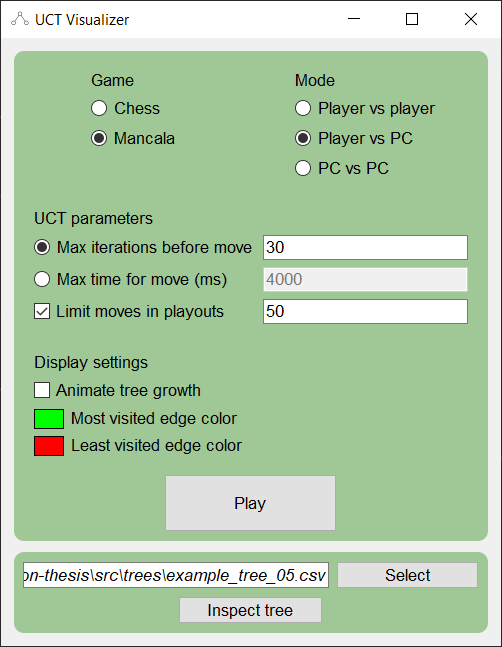
\includegraphics[width=0.45\textwidth]{main-app-window}
\end{center}
Dostępne funkcje:\\
\begin{enumerate}
	\item Wybór jednej z dwóch gier:
	\subitem $\bullet$ mancala
	\subitem $\bullet$ szachy.\\
	\item Wybór jednego z trzech trybów gry:
	\subitem $\bullet$ \textit{gracz vs PC} - po wykonanym ruchu gracza algorytm oblicza ruch komputera i wykonuje go
	\subitem $\bullet$ \textit{PC vs PC }- użytkownik decyduje, kiedy mają wykonać się ruchy komputera
	\subitem $\bullet$ \textit{gracz vs gracz} - rozgrywka dwóch graczy, co wiąże się z brakiem wizualizacji.\\
	\item Ustawienie parametrów ruchu algorytmu UCT:
	\subitem $\bullet$ ilość wykonanych iteracji - im więcej ich będzie, tym więcej razy powtórzone będą kroki symulacji kolejnego ruchu przez komputer, co przekłada się na jego większą dokładność i trafność. Minusem jest większy czas oczekiwania na wykonaniu ruchu. (przedział: 1-10000)
	\subitem $\bullet$ maksymalny czas na wykonanie ruchu przez komputer - opcja alternatywna dla powyższej. Zamiast podawać odgórnie ilość iteracji, użytkownik może podać czas, w jakim komputer będzie wyznaczał ruch. Po upłynięciu czasu ostatnia symulacja jest dogrywana. (przedział: 1000ms - 30000ms).\\
	\item Ucięcie iteracji po przekroczeniu arbitralnie ustalonej liczby ruchów danego ``playoutu'' (symulacji rozgrywki w obrębie iteracji). Opcja może być włączona lub wyłączona. Dla tego drugiego przypadku gra kończy się tylko wtedy, gdy symulacja gry zakończy się w naturalny sposób.\\
	\item Włączenie animacji rozrostu drzewa - pozwala obserwować jak zmieniało się drzewo w trakcie symulacji ruchu - drzewo wyświetlane jest po każdej iteracji algorytmu. W przypadku wybrania opcji maksymalnego czasu na wykonanie ruchu przez komputer ta opcja uwzględni również czas rysowania wszystkich drzew, co wiąże się ze stratą wydajności algorytmu.\\
	\item Wybór kolorów krawędzi - dla ruchów najczęściej i najrzadziej odwiedzanych przez algorytm. Kolory pozostałych krawędzi będą gradientami podanych kolorów - dla powyższego przykłądowego okna, krawędzie częściej odwiedzanych węzłów będą bardziej zielone i mniej czerwone.\\
	\item Wybór drzew do przeglądu - po kliknięciu przycisku \textit{Select} otwiera się dodatkowe okno, które prosi użytkownika o wybranie pliku bądź zestawu plików drzew do analizy. Przyjmowane będą pliki w formacie .csv i binarnym (.tree), w ktorych dane zapisane będą według ustalonego schematu. Zakładamy poprawność wczytywanych plików. W polu tekstowym wyświetli się wówczas ścieżka do wczytanego pliku lub liczba plików w przypadku wczytania ich większej liczby.\\
\end{enumerate}
Aby rozpocząć rozgrywkę, należy nacisnąć przycisk \textit{Play}. Aby wizualizować wczytane drzewa - \textit{Inspect tree}.
\subsection{Okno podglądu drzewa}
Okno to umożliwia wizualizację drzew z wczytanych plików oraz sprawne poruszanie się po niej, wraz z możliwością wyświetlania statystyk poszczególnych węzłów:
\begin{center}
	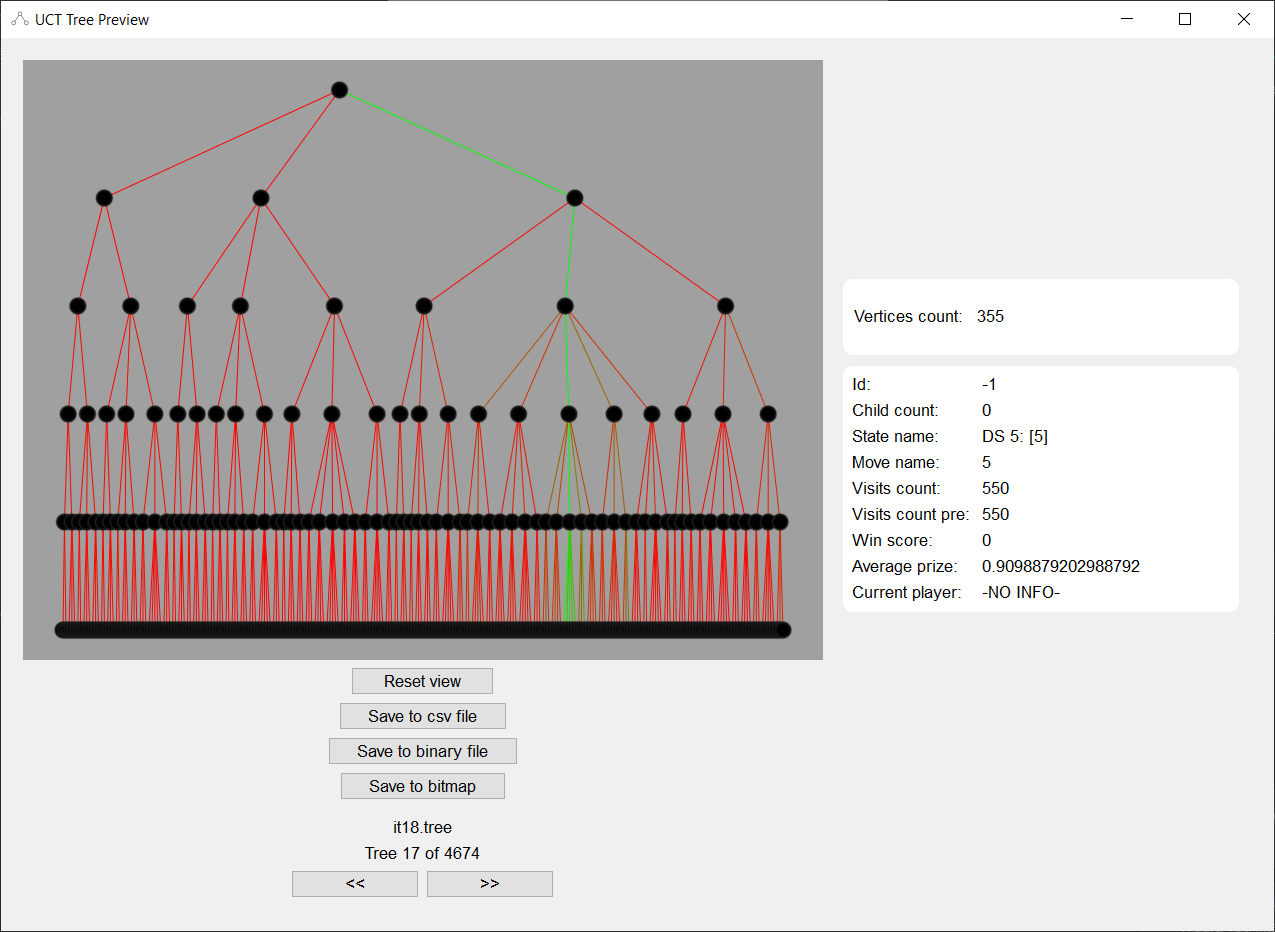
\includegraphics[width=0.8\textwidth]{tree-window}
\end{center}
Dostępne funkcje:\\
\begin{enumerate}
	\item Przybliżanie i oddalanie drzewa za pomocą scrolla. Kursor musi znajdować się nad częścią okna, gdzie wyświetlane jest drzewo.\\
	\item Przesuwanie drzewa - należy przytrzymać prawy przycisk myszy i poruszać myszką.\\
	\item Wyświetlenie statystyk węzła - należy kliknąć lewym przyciskiem myszy na dany węzeł. Po wybraniu węzła, po prawej stronie wyświetlają się jego statystyki:
	\subitem $\bullet$ ilość wszystkich wierzchołków drzewa
	\subitem $\bullet$ identyfikator węzłą
	\subitem $\bullet$ ilość węzłów-dzieci
	\subitem $\bullet$ nazwa stanu
	\subitem $\bullet$ nazwa ruchu
	\subitem $\bullet$ liczba odwiedzin węzła przez algorytm
	\subitem $\bullet$ suma wszystkich wygranych (łącznie wyniki poztywne i negatywne)
	\subitem $\bullet$ średnia wygrana - suma wygranych $\div$ ilość odwiedzin. Wartość z przedziału $[0, 1]$
	\subitem $\bullet$ numer gracza, który wykonał ruch dla danego węzła (1 lub 2).\\
	\item Wyśrodkowanie drzewa - resetuje stopień przybliżenie i przesunięcia.\\
	\item Zapis drzewa:
	\subitem $\bullet$ w formacie .csv
	\subitem $\bullet$ w formacie binarnym (.tree)
	\subitem $\bullet$ jako bitmapa (.png).\\
	\item Zmiana drzewa w sekwencji - możemy robić to za pomocą przycisków \textit{<<} i \textit{>>} na ekranie lub za pomocą strzałek na klawiaturze. Wyświetlana jest nazwa aktualnie przeglądanego pliku oraz to, którym jest on plikiem z kolei.\\
\end{enumerate}
Zamknięcie tego okna nie kończy programu - okno menu głównego jest ciągle aktywne i może być wykorzystane ponownie.

\subsection{Okno gry i wizualizacji}
Jest to połączenie gry oraz okna podglądu drzewa opisanego powyżej. Znajduje się tu interfejs graficzny toczącej się gry, w którą może ingerować użytkownik i wykonywać swoje ruchy. W górnej części znajduje się pasek postępu, który odzwierciedla ilość wykonanych przez algorytm iteracji podczas wyznaczania następnego ruchu. Po jego wyznaczeniu w środkowej częsci okna ukazuje się wygenerowane drzewo. Jeżeli użytkownik włączył opcję animacji drzew w menu głównym, dodatkowo po każdej iteracji będzie mógł on oglądać rozrost drzewa.\\
\begin{center}
	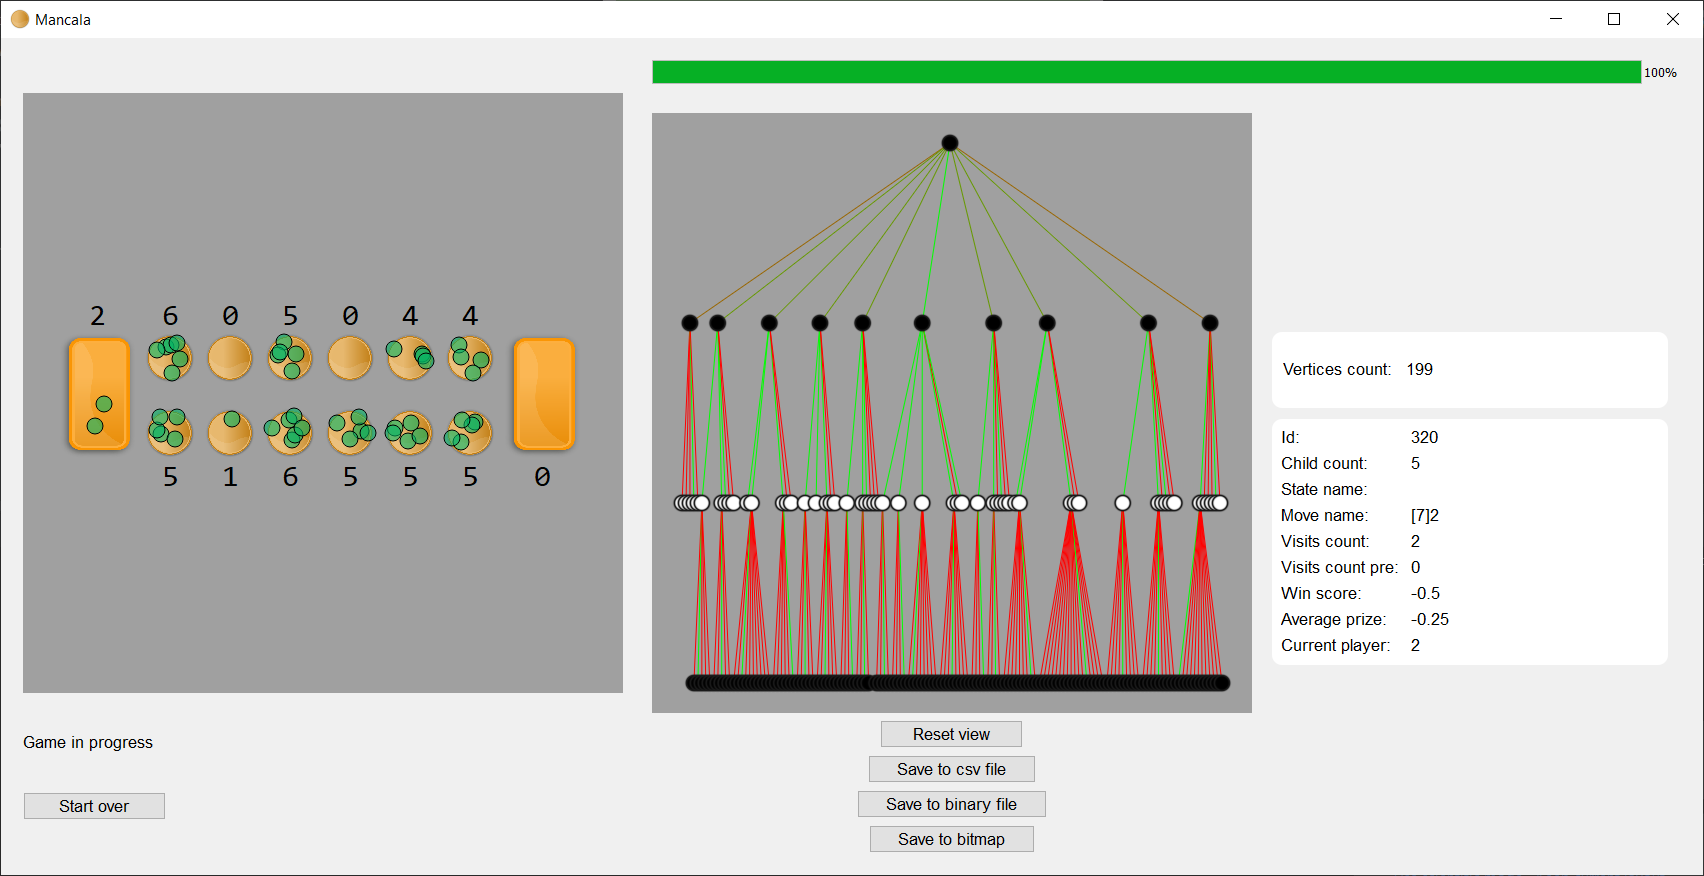
\includegraphics[width=\textwidth]{game-window}
\end{center}
Dostępne funkcje:\\
\begin{enumerate}
	\item Wszystkie funkcje dostępne w oknie podglądu drzewa poza sekwencjami.\\
	\item Wykonanie ruchu z pomocą GUI gry, np. kliknięcie danego pola w szachach lub dołka w mancali. Nie dotyczy trybu \textit{gracz vs PC}. Po zakończonej rozgrywce napis \textit{Game in progress} pod polem gry zmienia wartość i oznajmia użytkownikowi, która strona wygrała (lub czy jest remis).\\
	\item Rozegranie gry od nowa - kliknięcie przycisku \textit{Start over}.\\
	\item Wykonanie następnego ruchu za pomocą przycisku - tylko w trybie \textit{PC vs PC}. Pozwala na spowodowanie postępu w symulacji rozgrywki komputera z samym sobą. Ruchy za pomocą GUI są wówczas zablokowane.\\
\end{enumerate}
Zamknięcie tego okna również nie kończy programu - okno menu głównego jest ciągle aktywne i może być wykorzystane ponownie.

\section{Architektura systemu}
\section{Użyte technologie}
\end{document}
